\documentclass{article}


\usepackage{siunitx} % Provides the \SI{}{} and \si{} command for typesetting SI units
\usepackage{graphicx} % Required for the inclusion of images
\usepackage{natbib} % Required to change bibliography style to APA
\usepackage{amsmath} % Required for some math elements 
\usepackage{listings}
\usepackage{placeins}
\usepackage{color}
\usepackage{caption}
\setlength\parindent{0pt} % Removes all indentation from paragraphs

\lstset{frame=tb,
  language=Matlab,
  aboveskip=3mm,
  belowskip=3mm,
  showstringspaces=false,
  columns=flexible,
  basicstyle={\small\ttfamily},
  numbers=none,
  numberstyle=\tiny\color{gray},
  keywordstyle=\color{blue},
  commentstyle=\color{green},
  stringstyle=\color{red},
  breaklines=true,
  breakatwhitespace=true,
  tabsize=3}
%\renewcommand{\labelenumi}{\alph{enumi}.} % Make numbering in the enumerate environment by letter rather than number (e.g. section 6)


\title{Lab 3 \\ Analysis of a Car Suspension System} % Title

\author{Aneesh Malhotra \\ G00844135} % Author name

\date{\today} % Date for the report

\begin{document}

\maketitle % Insert the title, author and date


% If you wish to include an abstract, uncomment the lines below
% \begin{abstract}
% Abstract text
% \end{abstract}

%----------------------------------------------------------------------------------------
%	SECTION 1
%----------------------------------------------------------------------------------------

\section{Introduction}



% If you have more than one objective, uncomment the below:
\begin{description}
\item[Objective] \hfill \\
The objective of this lab is to analyze the behavior of a car suspension system using a linear mass-spring model. We analyze how the position of the car behaves as a function of the road.
\end{description}

\subsection{The Model} 
In this experiment we analyzed a linear model of a car suspension system by using a dampened mass-spring system. In a general mass-spring system, we use Newton's laws to find $$my''(t)  + k_d y'(t) + k_s y(t) = x(t).$$ Where $x(t)$ is the forcing input to the system. In our model, we look at $y(t)$ as the distance the wheel of the car is above level pavement, given a suspension system with a particular damping coefficient $k_d$ and a spring constant $k_s$. We extend the mass-spring model to dampen the vertical velocity of the car, or rather $y'(t) -x'(t)$ and the vertical position, $y(t) - x(t)$. Using these as the velocity and position in the damped mass-spring equation and normalizing, we see $$ y''(t) +\frac{k_d}{m} y'(t) + \frac{k_s}{m} y(t) = \frac{k_d}{m} x'(t) + \frac{k_s}{m}x(t).$$ This system has a transfer function given by $$\frac{\frac{k_d}{m}s + \frac{k_s}{m}}{s^2 + \frac{k_d}{m} s + \frac{ks}{m}}$$. In our simulations, we set $k_s = 10^5 N/m$, $m = 250$, and let $k_d$ vary.

\subsection{Pavement}
Using the model from above we analyze three cases: a curb, a pothole, and a wavy road.
\begin{enumerate}
\item We model a car going over a curb of height $A_1$ as $x(t) = A_1 u(t)$.
\item We model a car going through a pothole of depth $A_2$ and width $T$ as $ x(t) = -A_2 u(t) + A_2 u(t-T)$.
\item We model a car going over a wavy road of amplitude $A_3$ and period $T$ as $x(t) = A_3 \cos(\frac{2\pi t}{T}).$
\end{enumerate}

%----------------------------------------------------------------------------------------
%	SECTION 2
%----------------------------------------------------------------------------------------

\section{Main Body}

\subsection{Curb}

We began by analyzing the response of a car over a curb of height $\si{0.1m}$. Since we have a linear system, we use Matlab to simply find the step response, then scale it by our factor $A_1$. Additionally, we tested various damping coefficients $k_d$ in order to see which would provide the smoothest ride for the passenger. We tested this for $k_d =10^4$, $k_d = 2\cdot 10^4$, and $k_d = 5 \cdot 10^3$. Our results are plotted below.

\begin{figure}[!htbp]
\begin{minipage}{\linewidth}
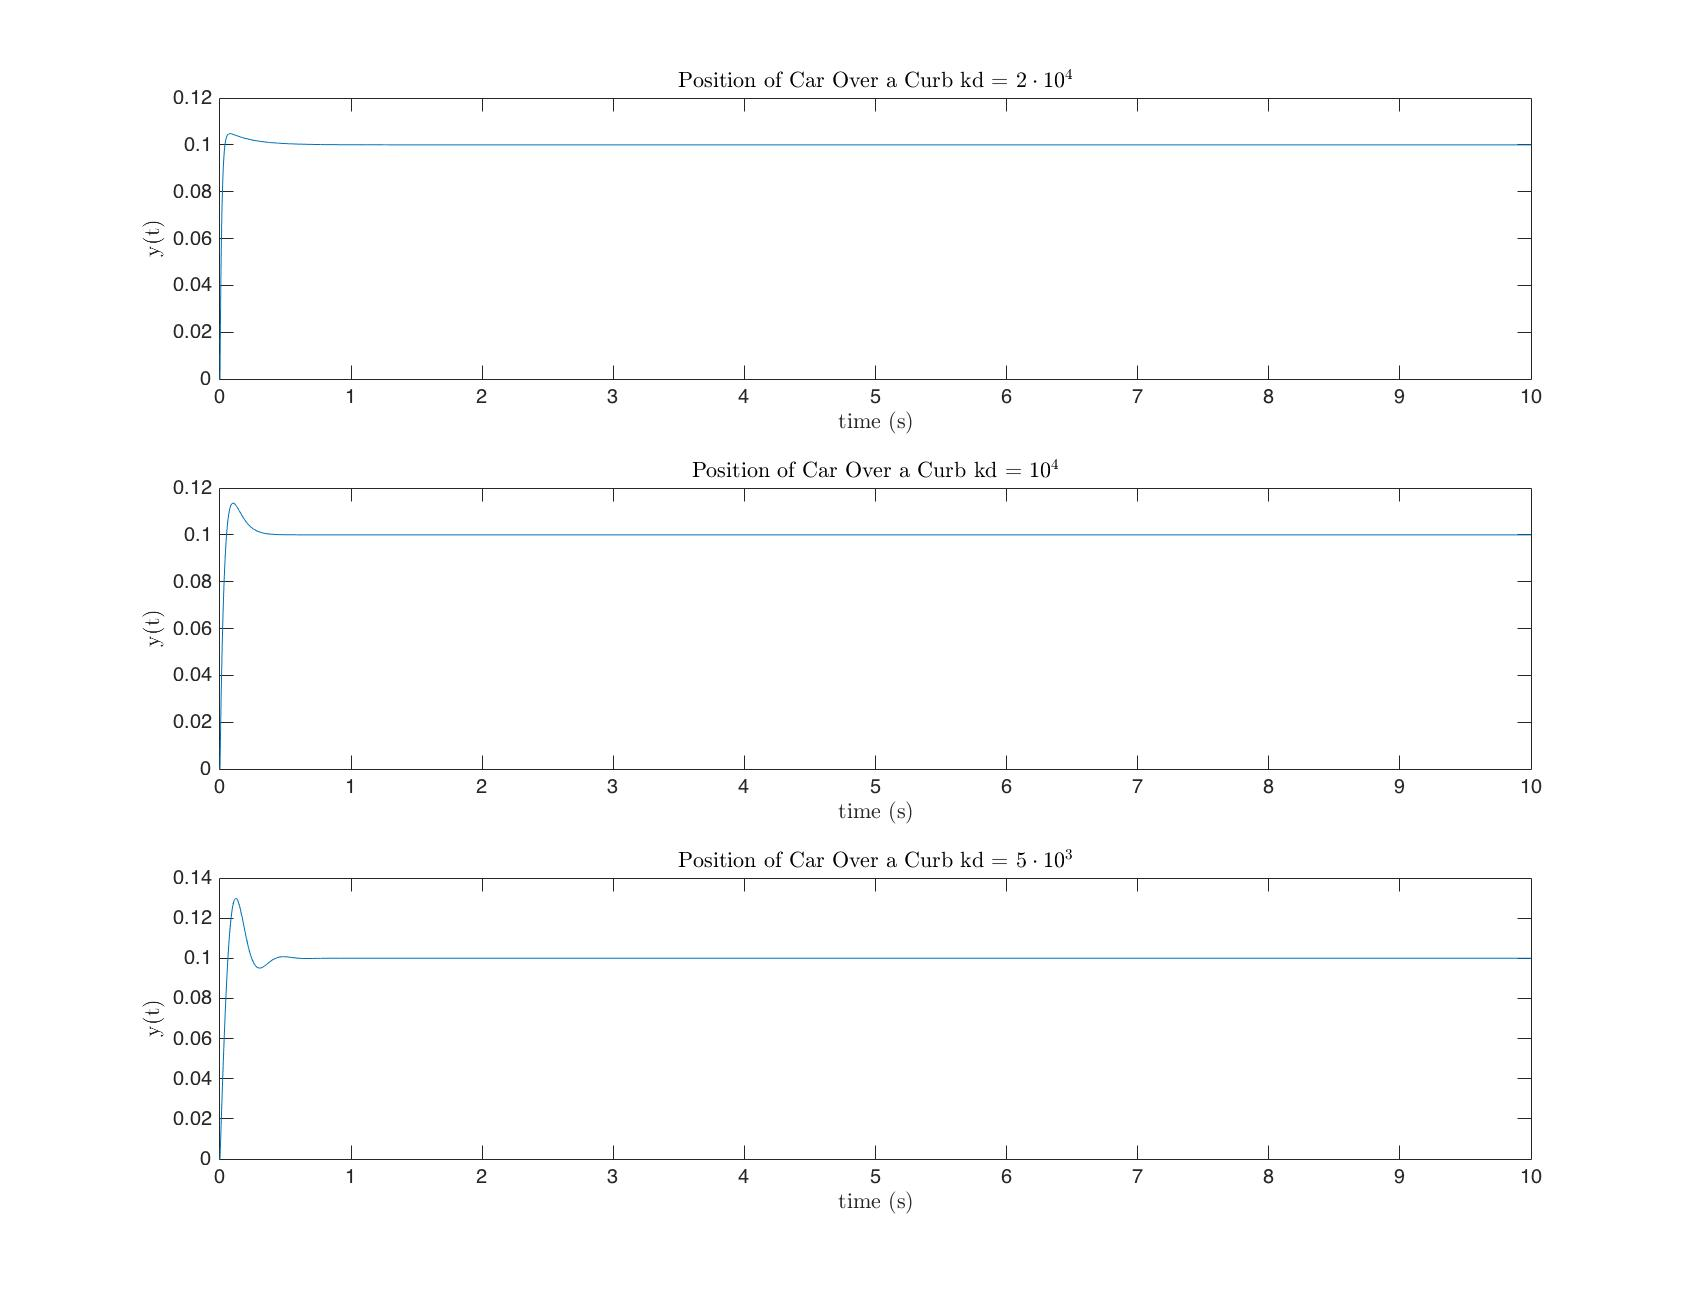
\includegraphics[width = 1\linewidth, height = 0.4\textheight]{curb.jpg}
\captionof{figure}{Response of a car going over a curb with varying damping coefficients}
\end{minipage}
\end{figure}

We see in the figure above that the higher damping constants lead to lower jumps in the vehicle, whereas the lower damping constants lead to higher jumps.
\FloatBarrier

\subsection{Pothole}
In this section we analyze what happens when we let $x(t)$ simulate a car going over a pothole of length $\si{1m}$ at $5\si{m/s}$. We see that in the time-domain, a wheel will traverse the pothole in $\frac{1}{5}$ $\si{s}$. We simulate this for $k_d$ values of $10^4$ and $2\cdot 10^3$. The plot is shown below.

\begin{figure}[!htbp]
\begin{minipage}{\linewidth}
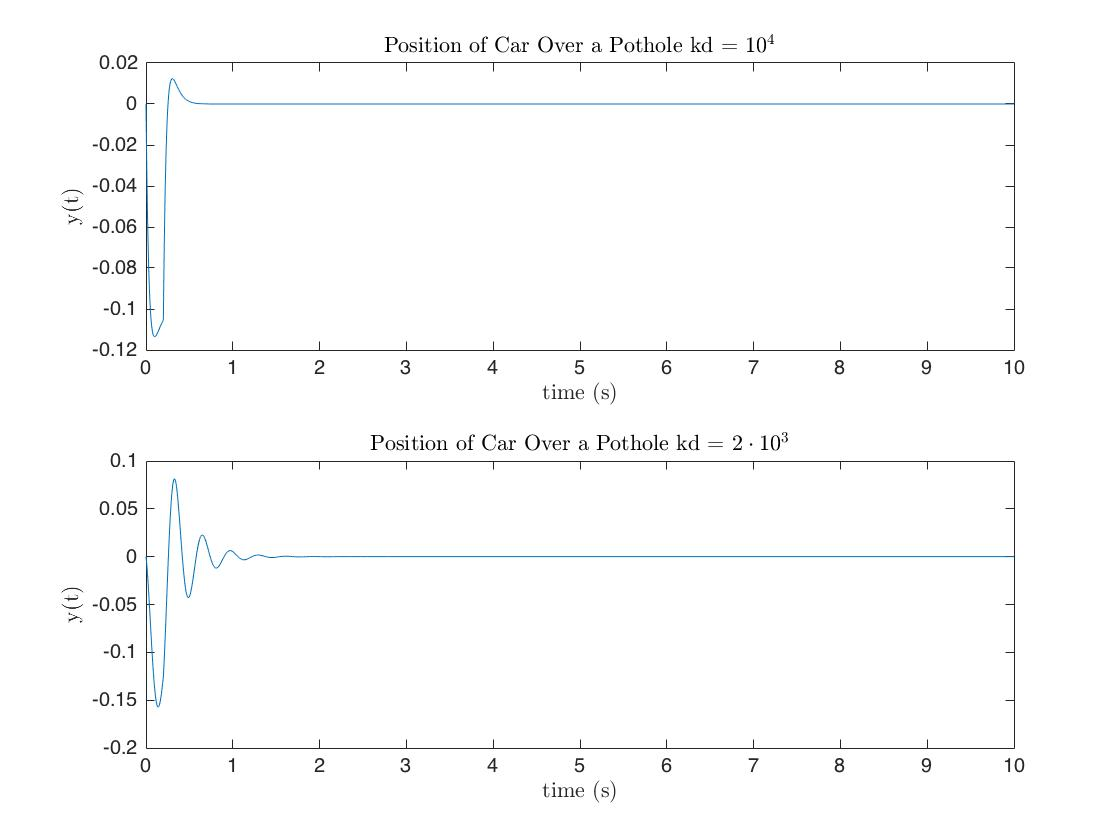
\includegraphics[width = 1\linewidth, height = 0.5\textheight]{pothole.jpg}
\captionof{figure}{Response of a car going over a pothole with varying damping coefficients}
\end{minipage}
\end{figure}


In this case it we see that the car with the lower damping coefficient tends to shake more after crossing the pothole than the car with the higher damping coefficient. 

\subsection{Wavy Road}
We finally model the case of a wavy road as a sinusoid given by $x(t) = A_3 \cos(2 \pi t/ T).$ In our case, the amplitude of the road is $5 \si{cm}$ and the period of the road is $0.314\si{s}$. The output is shown below for a $k_d$ value of $10^4$.

\begin{figure}[!htbp]
\begin{minipage}{\linewidth}
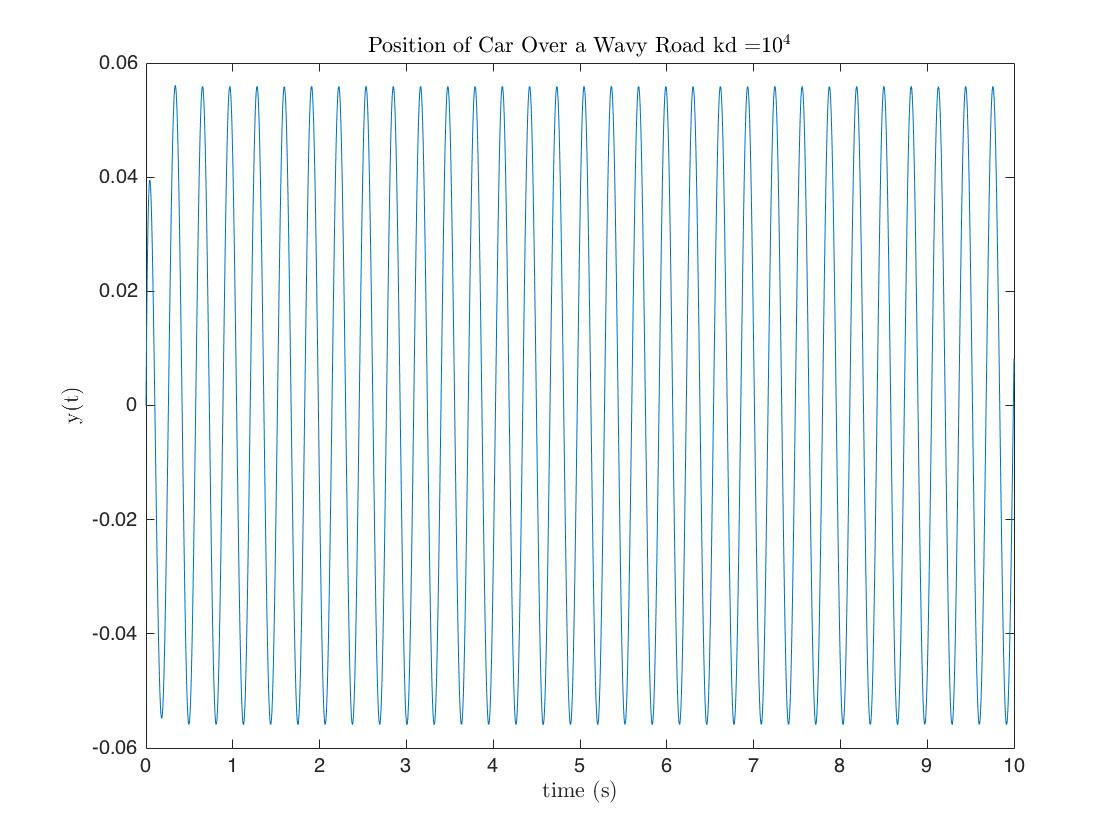
\includegraphics[width = 1\linewidth, height = 0.5\textheight]{wavy.jpg}
\captionof{figure}{Response of a car going over a wavy road}
\end{minipage}
\end{figure}
\FloatBarrier


In this case we initial damping when the car begins to go over the road, but the car eventually ends moving along in phase with the road. 

\section{Conclusion}
In this lab we studied three major cases. In the first two cases, we saw that higher damping coefficients were key in keep the car steady when running across disruptions the road. In the case of the curb, we saw that the car with the lowest damping coefficient depressed down before coming back up, creating a more bumpy ride whereas the car with the higher damping coefficients only rose and came back down. In the pothole case, the car with the lowest damping coefficient in the suspension kept bouncing for over a second after passing the pothole, whereas the one with higher damping went to equilibrium almost immediately. In the wavy road case, we only studied the $k_d = 10^4$ case and saw that there was only initial damping, but the car only moved along with the road. Overall, the model used was not entirely accurate, as you would expect in the case of curved motion, like in the sinusoidal case, there would be a force of gravity that would play a role in the net centripetal force felt by the car. Additionally, if the pothole or curb were too high, to resemble a wall or a ditch, we would not expect the car to keep moving with time.


\subsection{Code}
\lstinputlisting{Lab3.m}
%----------------------------------------------------------------------------------------
%	BIBLIOGRAPHY
%----------------------------------------------------------------------------------------
\section{References}

Lathi, B. P. Linear Systems and Signals. New York: Oxford UP, 2005. Print.

\end{document}